\documentclass{article}

\usepackage{amsmath}
\usepackage{dirtytalk}
\usepackage{float}
\usepackage{graphicx}
\usepackage{listings}

\setlength\parindent{0pt}

\begin{document}

    \title{HPCSE II - Exercise 3}
    \author{Anian Ruoss}
    \maketitle

    \section*{Part I}
    \label{sec:PartI}

    \begin{figure}[H]
        \begin{center}
            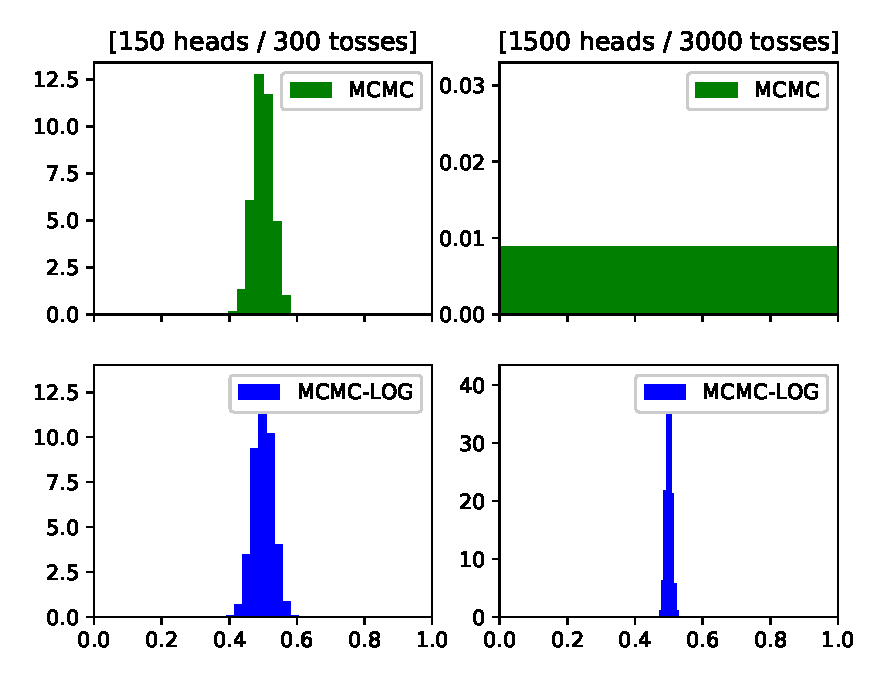
\includegraphics[width=.75\textwidth]{plots/coin_toss.eps}
        \end{center}
        \caption{Histogram of the posterior distribution
        $p \left( H | d \right)$ from the coin toss example sampled via
        Metropolis-Hastings MCMC.
        The top row samples are computed in the original scale and the
        bottom row samples are computed in the logarithmic scale.
        For a large number of tosses the MCMC in the original scale
        experiences overflow errors and thus fails to produce valid samples.
        In the logarithmic scale we observe that increasing the number of
        tosses (while keeping the number of heads and tails equal) reduces
        the variance of the posterior distribution as the prior is more
        certain that the coin is fair.
        }
    \end{figure}

    \section*{Part II}
    \label{sec:PartII}

    \subsection*{Task 1}
    \label{subsec:Task1}

    \subsubsection*{a)}
    \label{subsubsec:Task1a}

    \begin{lstlisting}[language=bash, basicstyle=\tiny, frame=single,
    caption={Korali output when determining the optimal x- and y-coordinates
    in terms of grass height.}, label={lst:KoraliOptGrassCoords}]
[Korali] Starting CMAES. Parameters: 2, Seed: 0x5C9F5947
...
[Korali] Parameter 'x' Value: 4.085200
[Korali] Parameter 'y' Value: 3.747600
[Korali] Total Elapsed Time: 0.002758s
    \end{lstlisting}

    \begin{lstlisting}[basicstyle=\tiny, frame=single,
    caption={Terminal output for $check\_cows$ with the optimal x- and
    y-coordinates determined in Listing~\ref{lst:KoraliOptGrassCoords}.},
    label={lst:CowsOptGrassCoords}]
Searching for cows near (4.085200, 3.747600)...
...
New cows found: 9
Total cows found so far: 9
Herr Kueheli says: "I knew we should look around the spot with the tallest grass!."
Herr Kueheli says: "The rest of the cows should be around here. Lets try these
nearby points:"
[4.08, 3.95]
[4.28, 3.75]
[3.88, 3.75]
[4.08, 3.55]
>>> Time until deadline: 55 minutes. <<<
    \end{lstlisting}

    \subsubsection*{b)}
    \label{subsubsec:Task1b}

    If the grass is high at one point it should be of roughly equal height in
    its immediate surroundings for a sufficiently \say{nice} (e.g.\
    continuous) function as we would expect grass growth to be from our
    experience in the real world.
    Thus Mr. Kueheli suggests to move roughly 200 meters along each axis
    (in both directions), as he can only see that far, and check if there
    are any more cows there.
    The suggested locations can be found in
    Listing~\ref{lst:CowsOptGrassCoords} and the corresponding $check\_cows$
    outputs are presented in listings~\ref{lst:CowsOptTopGrassCoords},
    \ref{lst:CowsOptRightGrassCoords},~\ref{lst:CowsOptLeftGrassCoords},
    and~\ref{lst:CowsOptBottomGrassCoords}.

    \begin{lstlisting}[basicstyle=\tiny, frame=single,
    caption={Terminal output for $check\_cows$ with one of the suggested x-
    and y-coordinates from in Listing~\ref{lst:CowsOptGrassCoords}.},
    label={lst:CowsOptTopGrassCoords}]
Searching for cows near (4.080000, 3.950000)...
...
New cows found: 15
Total cows found so far: 24
Herr Kueheli says: "That was good, but we need to find them faster!."
>>> Time until deadline: 50 minutes. <<<
    \end{lstlisting}
    \begin{lstlisting}[basicstyle=\tiny, frame=single,
    caption={Terminal output for $check\_cows$ with one of the suggested x-
    and y-coordinates from in Listing~\ref{lst:CowsOptGrassCoords}.},
    label={lst:CowsOptRightGrassCoords}]
Searching for cows near (4.280000, 3.750000)...
New cows found: 0
Total cows found so far: 24
Herr Kueheli says: "That was not good enough, perhaps this strategy does not really
                    work."
>>> Time until deadline: 45 minutes. <<<
    \end{lstlisting}
    \begin{lstlisting}[basicstyle=\tiny, frame=single,
    caption={Terminal output for $check\_cows$ with one of the suggested x-
    and y-coordinates from in Listing~\ref{lst:CowsOptGrassCoords}.},
    label={lst:CowsOptLeftGrassCoords}]
Searching for cows near (3.880000, 3.750000)...
...
New cows found: 1
Total cows found so far: 25
Herr Kueheli says: "That was not good enough, perhaps this strategy does not really
                    work."
>>> Time until deadline: 40 minutes. <<<
    \end{lstlisting}
    \begin{lstlisting}[basicstyle=\tiny, frame=single,
    caption={Terminal output for $check\_cows$ with one of the suggested x-
    and y-coordinates from in Listing~\ref{lst:CowsOptGrassCoords}.},
    label={lst:CowsOptBottomGrassCoords}]
Searching for cows near (4.080000, 3.550000)...
New cows found: 0
Total cows found so far: 25
Herr Kueheli says: "That was not good enough, perhaps this strategy does not really
                    work."
>>> Time until deadline: 35 minutes. <<<
    \end{lstlisting}

    We found another 16 cows which is roughly to be expected as cows tend to
    be where the grass is high which is roughly around the maximum as
    outlined above.
    Of course, we cannot expect all cows to be concentrated around this
    area as then they would eat all the grass and move on to other places.
    For this reason we assume the cows to be distributed around different
    areas of Mr. Kueheli's farm.


    \subsubsection*{c)}
    \label{subsubsec:Task1c}

    We use Korali's TMCMC sampling engine to gain a better understanding of
    the grass height distribution around the farm and display the results
    in Figure~\ref{fig:GrassHeight}.

    \begin{figure}[H]
         \begin{center}
            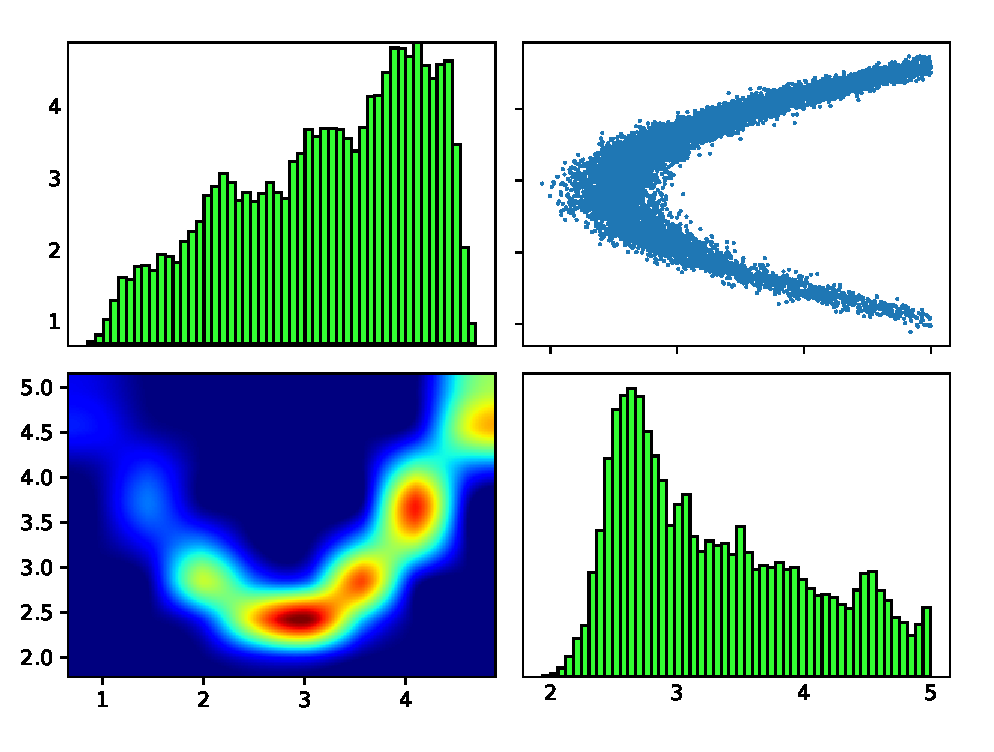
\includegraphics[width=.75\textwidth]{task1/results/task1c.eps}
        \end{center}
        \caption{Visualization of the grass growth distribution.
        We oberserve (local) maxima at roughly $\left( 4.08, 3 .75 \right)$
        (as obtained in Listing~\ref{lst:KoraliOptGrassCoords}) and
        $\left( 3, 2.5 \right)$.}
        \label{fig:GrassHeight}
    \end{figure}

    With this information we check for cows at the (local) maximum
    $\left( 3, 2.5 \right)$ and in its immediate surroundings (due to Mr.
    Kueheli's reasoning from above.) and we present the terminal outputs in
    listings~\ref{lst:CowsOpt},~\ref{lst:CowsOptRight},
    and~\ref{lst:CowsOptLeft}.

    \begin{lstlisting}[basicstyle=\tiny, frame=single,
    caption={Terminal output for $check\_cows$ for the coordinates of the
    (local) maximum observed in Figure~\ref{fig:GrassHeight}.},
    label={lst:CowsOpt}]
Searching for cows near (3.000000, 2.500000)...
...
New cows found: 90
Total cows found so far: 115
Herr Kueheli says: "Great, this strategy is really effective!."
>>> Time until deadline: 30 minutes. <<<
    \end{lstlisting}
    \begin{lstlisting}[basicstyle=\tiny, frame=single,
    caption={Terminal output for $check\_cows$ for a point in the
    neighborhood of the (local) maximum observed in
    Figure~\ref{fig:GrassHeight}.}, label={lst:CowsOptRight}]
Searching for cows near (3.200000, 2.500000)...
...
New cows found: 32
Total cows found so far: 147
Herr Kueheli says: "Great, this strategy is really effective!."
>>> Time until deadline: 25 minutes. <<<
    \end{lstlisting}
    \begin{lstlisting}[basicstyle=\tiny, frame=single,
    caption={Terminal output for $check\_cows$ for a point in the
    neighborhood of the (local) maximum observed in
    Figure~\ref{fig:GrassHeight}.}, label={lst:CowsOptLeft}]
Searching for cows near (2.800000, 2.500000)...
...
New cows found: 37
Total cows found so far: 184
Herr Kueheli says: "Thanks so much, you and Korali helped me find all my cows in
                    time!."
    \end{lstlisting}

    The initial strategy relied on the fact that enough cows could be found
    around the point of maximum grass height.
    However, the maximum only gives us a point estimate and no information
    about the underlying distribution of the grass growth (and thus no
    information about the grass height in the neighborhood of the global
    maximum).
    Thus by sampling the distribution, we were able to locate lager areas
    of high grass and correspondingly also more cows.
    In this concrete case, we observe that the global maximum has a
    relatively small neighborhood of high grass whereas other local maxima
    have larger areas of high grass surrounding them.
    Naturally, we expect more cows in larger areas of high grass (i.e.\ the
    local maximum) than in a small area with very high grass (i.e.\ the
    global maximum) as cows tend to value some personal space\footnote{This
    has been verified via personal communication with a large sample of cows.}.
    Of course, we don't know this before looking at the underlying distribution
    so the initial strategy is not the most efficient (of course, this
    assumes the we can actually sample from the distribution).

    \subsubsection*{d)}
    \label{subsubsec:Task1d}

    We can use Korali to investigate the posterior distribution of the
    parameters pH and mm given the grass growth and suitable priors.
    Naturally we model experts' clues as prior distributions of the pH and the
    rain volume.
    More concretely, we set $p(\text{pH}) \sim \mathcal{U}(4, 9)$ and
    $p(\text{mm}) \sim \mathcal{N}(90, 20)$.
    Korali requires us to set bounds for the Gaussian prior on mm.
    We choose the lower bound of $0$ (as we cannot have negative rain) and
    the upper bound of $180$ (for symmetry around the mean).
    Employing Korali's CMAES solver we maximize the posterior and we display
    the results in Listing~\ref{lst:MaxGrassPosterior}.

    \begin{lstlisting}[basicstyle=\tiny, frame=single, caption={Korali
    output when maximizing the posterior of the pH and mm parameters.},
    label={lst:MaxGrassPosterior}]
[Korali] Starting CMAES. Parameters: 3, Seed: 0x5C9D72B9
...
[Korali] Parameter 'Sigma' Value: 0.144379
[Korali] Parameter 'pH' Value: 7.472116
[Korali] Parameter 'mm' Value: 115.494066
[Korali] Total Elapsed Time: 0.006133s
    \end{lstlisting}

    We observe that both parameter values at the maximum of the posterior lie
    within the optimal range for pumpkins.
    However, the uncertainty --- as quantified by the value of $\sigma$ --- is
    rather high.
    For this, reason we sample from the posterior distribution of the
    parameters with Korali's TMCMC sampling engine to get a better estimate
    of the soil conditions and we display the results in
    Figure~\ref{fig:GrassPosterior}.

    \begin{figure}[H]
        \begin{center}
            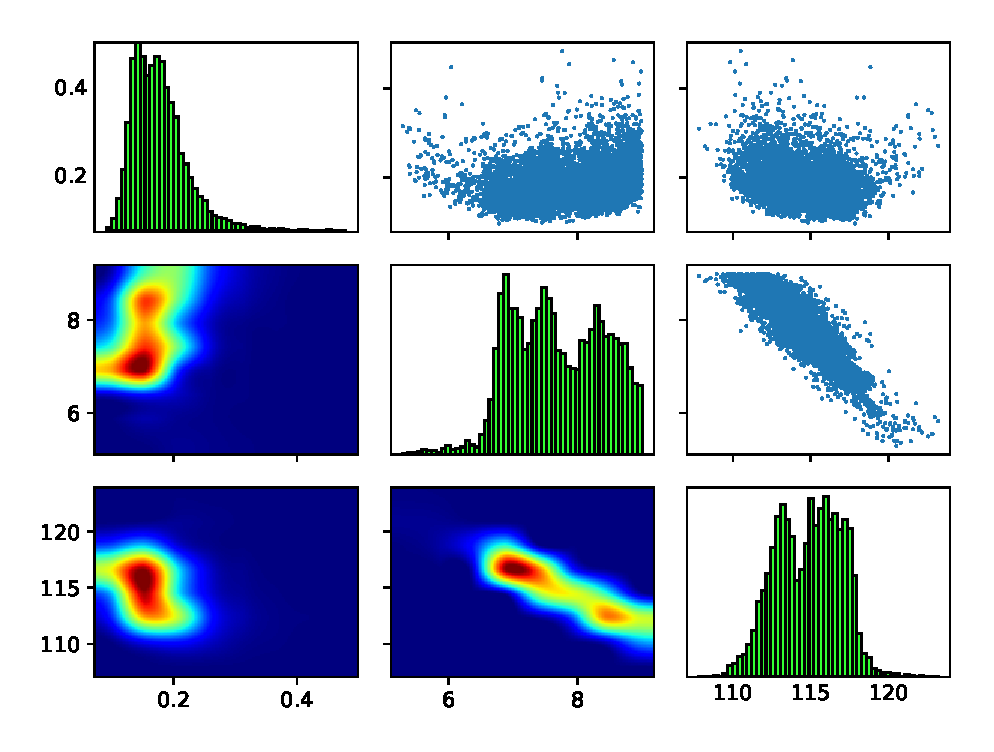
\includegraphics[width=.75\textwidth]{task1/results/task1d.eps}
        \end{center}
        \caption{Visualization of the posterior distribution of the
        parameters.
        The histogram in the center shows that the pH distribution is skewed
        to the right of $7.5$.
        The bottom-left histogram shows that the rain volume falls almost
        entirely within the range $\left[ 110, 120 \right]$.
        }
        \label{fig:GrassPosterior}
    \end{figure}

    We observe that there is very probably enough rain, i.e.\ more than
    $100mm$ per month.
    However, we also observe that the pH at the maximum of the posterior is
    atypical in the sense that it does not give us a good estimate of the pH
    distribution as it is very likely that the actual soil conditions will
    fall within the range $\left[ 7.5, 9 \right]$.
    Unfortunately, this means that we cannot fully recommend that Ms.
    Kleineblume plant pumpkins at this point of the year as the soil is
    probably to basic for her crop.

    \subsection*{Task 2}
    \label{subsec:Task2}

    \subsubsection*{a)}
    \label{subsubsec:Task2a}





\end{document}
